\documentclass[11pt,a4paper]{ivoa}
\input tthdefs

\usepackage{listings}
\lstloadlanguages{sh,make,[latex]tex}
\lstset{flexiblecolumns=true,numberstyle=\small,showstringspaces=False,
  identifierstyle=\texttt,defaultdialect=[latex]tex,language=tex}

\usepackage{todonotes}
\usepackage{float}
\usepackage{adjustbox}
\usepackage{lscape} 

\usepackage[english]{babel}

%Import the natbib package and sets a bibliography  and citation styles
\usepackage{natbib}
\bibliographystyle{abbrvnat}

\usepackage[utf8]{inputenc}

\usepackage{booktabs,xcolor,siunitx}
\definecolor{texcolor}{rgb}{0.4,0.1,0.1}
\definecolor{lightgray}{gray}{0.9}

\iftth
  \newcommand{\BibTeX}{BibTeX}
\fi

\newcommand{\comicstuff}[1]{
    \begin{html}<span class="comic">#1</span>\end{html}}
\customcss{custom.css}

\title{Observation Locator Table Access Protocol}

\ivoagroup{Data Model Working Group}

\author{Jesús Salgado}
\author{Aitor Ibarra}
\author{Matthias Ehle}
\author{Carlos Gabriel}
\author{James Dempsey}
\author{Markus Demleitner}
\author{María Díaz Trigo}
\author{Jaime Kennea}
\author{Mark Kettenis}
\author{Peter Kretschmar}
\author{Erik Kuulkers}
\author{Giorgio Matt}
\author{Bruno Merín}
\author{Marco Molinaro}
\author{Jan-Uwe Ness}
\author{Julian Osborne}
\author{Emma de Oña Wilhelmi}
\author{Edward J. Salbol}
\author{Emilio Salazar}
\author{Celia Sánchez}
\author{Richard Saxton}
\author{Gregory Sivakoff}
\author{Lian Tao}
\author{Aaron Tohuvavohu}
\author{Bill Workman}
\author{TBC: Representatives of a large multi-observatory collaboration}

\editor{Jesús Salgado}
\editor{Aitor Ibarra}


      
\begin{document}

\begin{abstract}
The \textbf{Observation Locator Table Access Protocol (ObsLocTAP) }document
describes the necessary data model elements and the access protocol to discover
metadata about observations for a given Astronomical Observatory through a
uniform interface within the VO framework. 

The used data model makes reference to IVOA Observation Data Model elements
(\cite{Lou17}), removing the ones associated to datasets access, as these
elements are not available yet for future observations that are planned,
scheduled, performed but not archived. In this way, present standard is focused
on the access to metadata related to the planning of a certain observatory, more
than in the access to the scientific data products of a certain observation.
Also, the data model described in the present standard will be focused on
metadata discovery, useful for multiwavelength coordination observations. However, 
and in order to prevent coupling between ObsCore and ObsLocTAP standards, ObsLocTAP 
defines its own data model.

The access protocol will be expressed by the implementation of an IVOA Table Access 
Protocol (TAP) (\cite{Pat10}), that, as described in the use cases, allows a powerful 
discovery process and, also, the implementation of the use cases proposed in the 
present specification.

\textbf{ObsLocTAP} services could be registered using a TAP VOResource Extension 
(\cite{Dem15}) providing the relevant ObsLocTAP capability. Exact details of the 
VOResource Extension will be defined in another appropriate standard definition.

In the case of a simple use case, planned observations of a certain target can be 
discovered via a TAP and ADQL (\cite{Ina08}) query that searches for sky regions 
(or FOV) that overlap a certain sky coordinate. Adding a certain radius to the sky 
coordinates and/or filtering by instrument identifier could expand this simple use 
case.

As described in TAP, the service will return a list of performed observations of 
the given target and also the future planned and/or scheduled observations in 
VOTable (\cite{Fra13}) format or, optionally, in other tabular serialization 
format, e.g., JSON. 

The information about the planned observation, in the near future, will be subject 
to changes due to any operational issue (re-planning, ToO alerts, etc). Thus, an 
implementation of the service may support additional search parameters (some of 
which may be custom to that particular service) to more finely control the selection 
of the observation information.
\end{abstract}

\section*{Acknowledgments}
The authors acknowledge the comments from Observatories members and from the IVOA 
members in general.


\section*{Conformance-related definitions}

The words ``MUST'', ``SHALL'', ``SHOULD'', ``MAY'', ``RECOMMENDED'', and
``OPTIONAL'' (in upper or lower case) used in this document are to be
interpreted as described in IETF standard RFC2119 (\citep{std:RFC2119}).

The \emph{Virtual Observatory (VO)} is a
general term for a collection of federated resources that can be used
to conduct astronomical research, education, and outreach.
The \href{http://www.ivoa.net}{International
Virtual Observatory Alliance (IVOA)} is a global
collaboration of separately funded projects to develop standards and
infrastructure that enable VO applications.

\section*{Link to IVOA Architecture}
The figure below shows where ObsLocTAP protocol fits within the IVOA architecture:

%%%%%%%%%%%%%%%%%%%% Figure/Image No: 1 starts here %%%%%%%%%%%%%%%%%%%%

\begin{figure}[H]
\advance\leftskip 0.0in	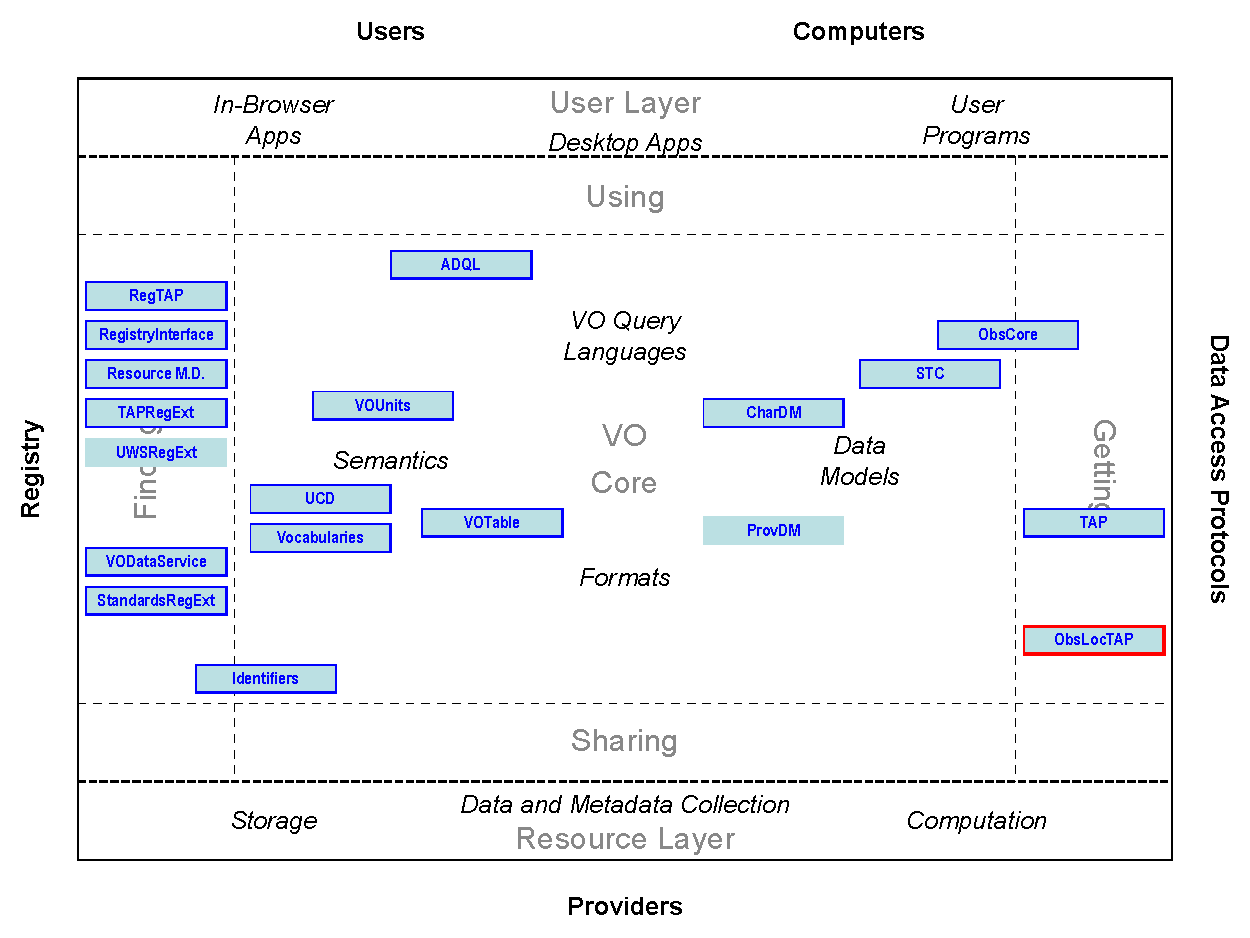
\includegraphics[width=6.0in,height=4.73in]{./role_diagram.pdf}
\end{figure}


%%%%%%%%%%%%%%%%%%%% Figure/Image No: 1 Ends here %%%%%%%%%%%%%%%%%%%%

\pagebreak
\vspace{\baselineskip}
{\fontsize{16pt}{19.2pt}\selectfont \textbf{\textcolor[HTML]{005A9C}{Change Log}}\par}\par



%%%%%%%%%%%%%%%%%%%% Table No: 2 starts here %%%%%%%%%%%%%%%%%%%%


\begin{table}[H]
 			\centering
\begin{tabular}{p{3.75in}p{0.92in}p{0.8in}}
\hline
%row no:1
\multicolumn{1}{|p{3.75in}}{\textbf{Change}} & 
\multicolumn{1}{|p{0.92in}}{\textbf{Section}} & 
\multicolumn{1}{|p{0.8in}|}{\textbf{Date}} \\
%row no:2
\multicolumn{1}{|p{3.75in}}{First Version} & 
\multicolumn{1}{|p{0.92in}}{All} & 
\multicolumn{1}{|p{0.8in}|}{{\fontsize{10pt}{12.0pt}\selectfont 20180710}} \\
%row no:3
\multicolumn{1}{|p{3.75in}}{Service renamed to ObsLocTAP} & 
\multicolumn{1}{|p{0.92in}}{All} & 
\multicolumn{1}{|p{0.8in}|}{{\fontsize{10pt}{12.0pt}\selectfont 20180713}} \\
%row no:4
\multicolumn{1}{|p{3.75in}}{Typos} & 
\multicolumn{1}{|p{0.92in}}{All} & 
\multicolumn{1}{|p{0.8in}|}{{\fontsize{10pt}{12.0pt}\selectfont 20180904}} \\
%row no:5
\multicolumn{1}{|p{3.75in}}{Data model re-definition (introduction of ivoa:obsplan ) \par Better definition of $``$category$"$  and $``$Priority$"$ } & 
\multicolumn{1}{|p{0.92in}}{All} & 
\multicolumn{1}{|p{0.8in}|}{{\fontsize{10pt}{12.0pt}\selectfont 20180913}} \\
%row no:6
\multicolumn{1}{|p{3.75in}}{Adding better distinction between planned, scheduled, performed and archived observations} & 
\multicolumn{1}{|p{0.92in}}{All} & 
\multicolumn{1}{|p{0.8in}|}{{\fontsize{10pt}{12.0pt}\selectfont 20190215}} \\
%row no:7
\multicolumn{1}{|p{3.75in}}{Correction of s\_fov as a circle radius. Possible use of more complex footprints as objects to be defined} & 
\multicolumn{1}{|p{0.92in}}{All} & 
\multicolumn{1}{|p{0.8in}|}{{\fontsize{10pt}{12.0pt}\selectfont 20190215}} \\
%row no:8
\multicolumn{1}{|p{3.75in}}{Introduction of s\_region to cover more complex footprints} & 
\multicolumn{1}{|p{0.92in}}{All} & 
\multicolumn{1}{|p{0.8in}|}{{\fontsize{10pt}{12.0pt}\selectfont 20190802}} \\
%row no:9
\multicolumn{1}{|p{3.75in}}{Many typos correction} & 
\multicolumn{1}{|p{0.92in}}{All} & 
\multicolumn{1}{|p{0.8in}|}{{\fontsize{10pt}{12.0pt}\selectfont 20190802}} \\
%row no:10
\multicolumn{1}{|p{3.75in}}{Use cases upgrade} & 
\multicolumn{1}{|p{0.92in}}{4} & 
\multicolumn{1}{|p{0.8in}|}{{\fontsize{10pt}{12.0pt}\selectfont 20190802}} \\
%row no:11
\multicolumn{1}{|p{3.75in}}{Add registering description} & 
\multicolumn{1}{|p{0.92in}}{5} & 
\multicolumn{1}{|p{0.8in}|}{{\fontsize{10pt}{12.0pt}\selectfont 20190802}} \\
%row no:12
\multicolumn{1}{|p{3.75in}}{Migration to LaTeX/github} & 
\multicolumn{1}{|p{0.92in}}{All} & 
\multicolumn{1}{|p{0.8in}|}{{\fontsize{10pt}{12.0pt}\selectfont 20200514}} \\
\hline
\end{tabular}
 \end{table}

\pagebreak

%%%%%%%%%%%%%%%%%%%% Table No: 2 ends here %%%%%%%%%%%%%%%%%%%%


\section{Overview}
The \textbf{Observation Locator Table Access Protocol} (ObsLocTAP henceforth) specifies 
in a standard format services to retrieve information about planned, scheduled and 
performed observations of a given target (or coordinates) for a given astronomical 
observatory based 
on the existing ObsCore data model. This standard does not describe the access to data 
obtained after the processing of the observational activity, as that is the goal of 
ObsCore (archived observations), although the discovery could be done in a similar way. 
Therefore, although there is some overlap on the data model described in both standards, 
entities, use cases and communities are different.

In order to standardize the workflow of one observation, status is defined as follows:
%%%%%%%%%%%%%%%%%%%% Figure/Image No: 0 starts here %%%%%%%%%%%%%%%%%%%%

\begin{figure}[H]
\advance\leftskip 0.0in		\hfill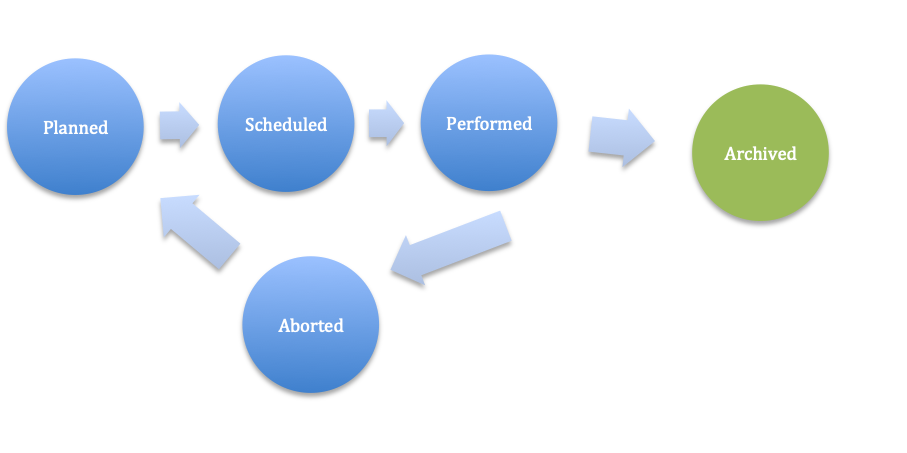
\includegraphics{./media/observations_workflow.png}\hfill\strut%
\end{figure}
%%%%%%%%%%%%%%%%%%%% Figure/Image No: 1 starts here %%%%%%%%%%%%%%%%%%%%

\begin{itemize}
	\item \textbf{Planned}: a possible observation, in most of the cases coming from a certain proposal, has been identified. There is not yet an association to a certain time period when the observation can be executed.

	\item \textbf{Scheduled}: mission planners allocate a certain period when the 
	observation can be executed. Also, some changes could be expected on coordinates 
	(due to some refinement) and other fields.

	\item \textbf{Performed}: the observation has been performed successfully. This is only at the operational level as there is not guarantee of scientific results.

	\item \textbf{Aborted}: the observation has not been correctly performed (or removed from the schedule). The observation could be recovered as planned into the planning log.

	\item \textbf{Archived}: the observation has data available and can be found in a science archive. This archived phase is the main target of the ObsCore specification, so it can be considered out of the scope of the present specification.
\end{itemize}

This service would allow client applications to use a standardized VO service to aggregate 
and display the information of former and future observations. This new standard will help 
inthe preparation of multi-observatory multi-instrument observation campaigns, whose 
coordination needs certain standards for efficient communication.

The ObsLocTAP interface makes use of the IVOA TAP (\cite{Pat10}) to access observational
metadata. The IVOA TAP protocol is a powerful and quite flexible system, easy to beadapted 
to different use cases by only having an agreed data model and the definition of a set of 
ADQL (\cite{Ina08}) queries that allow the implementation of different use cases. There 
are several open source implementations that could be used by the community (minimizing 
the implementation effort for the observatories) and it has been efficiently used in 
operational archives like, e.g., the Gaia Archive.

Making use of TAP, the following requirements of ObsLocTAP need to be fulfilled:

\begin{itemize}
	\item queries encoded as URLs\par

	\item query language based on ADQL defines the way to express geometrical queries and other filters as numeric ranges and value lists, 

	\item the use of VOTable for encoding search results,

	\item the mechanism for handling errors
\end{itemize}

Exact definition of the TAP service and functionality is present into the relevant IVOA 
standards (TAP and ADQL). In current document, we will focus the description of the Data 
Model, tables and use cases. No deviation from standard TAP or ADQL is foreseen.

\section{Use cases}
The planning process can be usually described as follows (although observatories can 
have different procedures to fulfill this process): 

\begin{itemize}
	\item The observatory receives observatory proposals from scientists that are reviewed by an expert panel (e.g., OTAC = Observing Time Allocation Committee). \par

	\item Proposals are ranked by their scientific relevance.

	\item Proposals are related to one or more observations that are inserted into the observation planning system of the observatory.

	\item Observation planners decide which observations can be scheduled in the short-medium plan trying to maximize the relevance of a certain observation period (e.g., per night or orbit revolution) and taking into account the constraints of the observatory (e.g., visibility of the object, geometrical constrains like the Sun or the Earth for space-based observatories, etc).

	\item In case of unexpected events like, e.g., targets of opportunity, the scheduled plan could be replaced by another one modifying the short or medium-term plans.
\end{itemize}

Standardizing the way to publish this short/medium plan through ObsLocTAP services provides 
higher scientific impact of the observing time, follow-up of astronomical events and 
better cooperation between observatories. We present here a selected list of user cases. 
Later in the document, we will show how these use cases can be fulfilled using the current specification:

\subsection{Common tooling for observers across observatories}
Standardization of the publication of observing plans will facilitate the implementation 
of a tool that lets observers monitor the progress of their proposed observations that 
works for all observatories that adopt ObsLocTAP. This kind of application has been 
requested by the community for a long time. Ideally, that would obviate custom, 
per-observatory web forms, saving work for observatories and observers alike. 

\subsection{Avoiding unnecessary proposals for observation time}
An astronomer wants to propose an observation and can, before doing so, globally 
determine if a possibly suitable observation is already scheduled.  This might prevent 
costly duplicate observations. 

\subsection{Support for weighting proposals}
The bodies (e.g., OTAC) that decide on the observation schedule can use the observation 
schedules of their own and other observatories to raise or lower priorities on a given 
proposal. This might even take into   account observation histories, giving demerits to 
possibly unnecessary   repeated observations.

\subsection{Identification of planned observations in a certain spectral range for a certain astronomical event}
A scientist could be interested in the planned observations for a certain astronomical 
object at different spectral ranges. For example, this is commonly done in the GRB 
(Gamma Ray Burst) events follow-up, where the event is decreasing in energy and multiple 
observations must be done in decreasing energy order by different observatories to fully 
characterize the event.

By using ObsLocTAP services, users could discover and propose sequential observations 
that will allow the future SED characterization of this astronomical event.

\subsection{Follow-up of Targets of Opportunity}
Observing plans can be changed very fast due to targets of opportunity (ToOs).

There are two different types of ToOs in astronomy:
\begin{itemize}
	\item Unpredictable ToOs: Astronomical events that require immediate or almost immediate observations and that may even require coordination between different observatories.

	\item Predictable ToOs: These astronomical events are related (not always) to known transient phenomena or due to coordinated observations of targets special interest. 
\end{itemize}

For the first type, the short-term plan can be affected in a very short time scale, as 
when they trigger follow-up observations of a certain astronomical event.

VOEvent initiatives are focused on the announcement of the astronomical event and in 
the propagation of the information obtained due to follow-up observations, but only 
when the observations are already executed. By the implementation of ObsLocTAP services, 
the decision how short-term observing plans are modified can be published live to the 
scientific community.

\subsection{Modification of the plans due to external conditions or anomalies}
Usually, observatory plans can be modified due to various reasons. They could be 
changed by anomalies in the instruments, astronomical events, external conditions, etc. 
For ground-based observations, atmospheric conditions could imply the modification 
of the planning, whereas for space-based observatories, radiation due to solar flares 
could force observations to be stopped.

It is difficult for the scientist to follow-up the status of the plan. This could be 
fulfilled by the implementation of ObsLocTAP services.

\section{Observation Locator Elements}
\subsection{Observation Locator data model }
In the IVOA ObsCore specification, two main data models are connected to describe the 
data model behind most of the use cases needed to discover observed datasets:

\begin{itemize}
	\item Characterization: Provides a description of metadata associated to a certain observation. In particular, the different axes (e.g., the spatial axis, the time axis, spectral axis$ \ldots $ ) are used to describe the coverage of the observation on different observables.
	\item ObsDataSet: Provides support to discover data associated to a certain performed observation.
\end{itemize}

In the case of planned (not executed) observations, only the Characterization DM could be
used, as the observations covered are not yet performed and hence most of the metadata 
associated to the ObsDataSet will be empty. Also, the data produced after the 
processing of the observational metadata could be not present yet for recently executed 
observations and, in other cases, data could be present only within the mission archive 
but not in the planning system. 

Although it is correctly set in the ObsCore DM that the association multiplicity 
between the Characterization DM and ObsDataSet is $0\ldots\ast$, the ObsCore 
specification clearly considers that metadata related to the data access is set for 
all the records. In the present document the data access metadata will not be included.

Also, although some of the elements could be known a priori, it is difficult to 
estimate the number of elements in the different axes (space, time, spectral,\dots). 
This implies that this information will not be present for most of the planning lists. 
This is why this information has been removed as well from the present data model.

That implies the data model for the use cases described in the present document is 
reduced to:

%%%%%%%%%%%%%%%%%%%% Table No: 3 starts here %%%%%%%%%%%%%%%%%%%%
\begin{landscape}
\begin{table}
\begin{tabular}{ |l|l|l|l| }
\hline
\textbf{Column Name} & 
\textbf{Unit} & 
\textbf{Type} & 
\textbf{Description} \\
\hline
%row no:2
t\_planning & 
d & 
double & 
Time in MJD when this observation has been added or modified into the planning log \\
\hline
%row no:3
target\_name & 
unitless & 
String & 
Astronomical object observed, if any \\
\hline
%row no:4
obs\_id & 
unitless & 
String & 
Observation ID \\
\hline
%row no:5
obs\_collection & 
unitless & 
String & 
Name of the data collection \\
\hline
%row no:6
s\_ra & 
deg & 
double & 
Central right ascension, ICRS \\
\hline
%row no:7
s\_dec & 
deg  & 
double & 
Central declination, ICRS \\
\hline
%row no:8
s\_fov  & 
deg & 
double & 
Diameter (bounds) of the covered region \\
\hline
%row no:9
s\_region & 
& 
String & 
Sky region covered by the data product (expressed in ICRS frame) \\
\hline
%row no:10
s\_resolution & 
arcsec & 
double & 
Spatial resolution of data as FWHM \\
\hline
%row no:11
t\_min & 
d & 
double & 
Start time in MJD \\
\hline
%row no:12
t\_max & 
d & 
double & 
Stop time in MJD \\
\hline
%row no:13
t\_exptime & 
s & 
double & 
Total exposure time \\
\hline
%row no:14
t\_resolution & 
s & 
double & 
Temporal resolution FWHM \\
\hline
%row no:15
em\_min & 
m & 
double & 
Start in spectral coordinates \\
\hline
%row no:16
em\_max & 
m & 
double & 
Stop in spectral coordinates \\
\hline
%row no:17
em\_res\_power & 
unitless & 
double & 
Spectral resolving power \\
\hline
%row no:18
o\_ucd & 
unitless & 
String & 
UCD of observable (e.g., phot.flux.density, phot.count, etc.) \\
\hline
%row no:19
pol\_states & 
unitless & 
String & 
List of polarization states or NULL if not applicable \\
\hline
%row no:20
pol\_xel & 
unitless & 
integer & 
Number of polarization samples \\
\hline
%row no:21
facility\_name & 
unitless & 
String & 
Name of the facility used for this observation \\
\hline
%row no:22
instrument\_name & 
unitless & 
String & 
Name of the instrument used for this observation \\
\hline
%row no:23
obs\_release\_date & 
unitless & 
date & 
Observation release date (ISO 8601) \\
\hline
%row no:24
t\_plan\_exptime & 
s & 
double & 
Planned or scheduled exposure time \\
\hline
%row no:25
category & 
unitless & 
String & 
Observation category (fixed, coordinated, etc...) \\
\hline
%row no:26
priority & 
unitless & 
enum integer & 
Priority level $ \{ $ 0, 1, 2$ \} $ \\
\hline
%row no:27
execution\_status & 
unitless & 
String & 
One of the following values:  Planned, Scheduled, Performed, Aborted \\
\hline
\end{tabular}
\end{table}
\end{landscape}

%%%%%%%%%%%%%%%%%%%% Table No: 3 ends here %%%%%%%%%%%%%%%%%%%%

The purpose of the observation locator query is to allow users/clients to retrieve the 
information of planned observations of a particular target or sky coordinates. The most 
basic query parameters will be the sky coordinates (Right Ascension and Declination). 
Additional parameters may be used to customize the visibility checks.

As can be seen, most of the data model elements come from the IVOA Characterization 
data model and the exact description of these fields is present in the IVOA ObsCore 
standard (\cite{Lou17}).

\textbf{\textit{s\_region}}, as described on IVOA ObsCore standard, can be used to 
precisely specify the covered spatial region of a data product. On the SELECT part, 
the output is always an STC-S string as described in (\cite{TAP}) [section 6]. In the 
WHERE clause, the \textit{s\_region} column can be used with the ADQL geometry functions 
(INTERSECTS, CONTAINS) to specify conditions; the service will generally have to translate 
these into native SQL that enforces the same conditions or a suitable approximation. 
Implementers may approximate the spatial query conditions by translating the INTERSECTS 
and CONTAINS function calls in the query. In case the exact final region cannot be 
specified (e.g., because an undefined position angle of the planned observation), 
s\_region will be just a CIRCLE with the center position as \textbf{s\_ra} and \textbf{s\_dec} 
and a radius of \textbf{s\_fov}/2.

The planning time (\textbf{t\_planning}) has been added in order to allow the discovery 
of the time when this observation (scientific entity) has been added (or modified) to 
the plan, in order to let clients ask for changes in the plan incrementally (i.e., 
without having to retrieve and compare locally the full set of future observations 
with a previously download one).

The planning exposure time (\textbf{t\_plan\_exptime}) has been added in order to 
show any possible inconsistency between the scheduled exposure time and the real 
performed exposure time (t\_\textbf{exptime}). If an observation was performed without 
problems, both quantities must be exactly the same. Any discrepancy between these two 
values will reflect problems or deviations between scheduled observations and performed 
observations.

The \textbf{category} element has been added in order to help users to identify those 
observations that were scheduled in coordination with other facilities or those 
observations that have to be executed at a fixed time.

The \textbf{priority} element has been added in order to help users to identify those 
observations that were scheduled with a high priority (value=2) and therefore cannot be 
removed from the planning or are hard to re-schedule. If the observation can be easily 
shifted to a different time (value=0), the user could query the service to identify this 
type of observations.

Execution status provides a description of the current status of the planned observation. 
Initially, observations are inserted as planned into the system. The final state will 
be one of executed or aborted.

\subsection{Compulsory metadata}
In contrast to normal ObsTAP services where most of the metadata is compulsory, in the 
case of ObsLocTAP, this cannot always be maintained. In some cases, the target associated 
to the observations could still be confidential information which needs to be hidden. 
This hidden identification of future observations is not always applicable for all the 
observatories but it is not so unusual. The same approach of hidden information status 
could also be applied to the instruments or configurations used so the metadata should 
be present as follows:

\begin{itemize}
	\item For confidential observations that need to be hidden from the planning point of view, the period should be shown as blocked. That means that an entry should appear with the start time, end time and duration as relevant. The facility name should also be provided.

	\item If the astronomical target is still hidden, coordinates and target should be set to \textit{null} in the obsplan table.

	\item Observational metadata about instrument, spectral coverage and polarization states should appear with a general default value, describing a non-detailed mode, but with values that are more general for the exact ones to be used during the real observation. For example, a general X-ray spectral coverage could appear in \textit{em\_min} and \textit{em\_max} for an X-ray observatory but not the exact details of the instrument mode that will be used for the confidential observation.

	\item Exact details of the observation could be updated whenever the observation passes from the hidden state to the public state from the metadata point of view.
\end{itemize}

\subsection{Implementation of ObsLocTAP as a TAP service}
In order to allow a powerful publication of the ObsLocTAP metadata, it has been decided to 
publish it through a TAP service. As described into the IVOA TAP standard (\cite{Pat10}), 
a TAP service is a web-service that allows the access to tabular data.\par

In order to fulfill some advanced use cases, ObsLocTAP services MUST provide, at least, the 
following ADQL (\cite{Ina08}) geometrical features: CIRCLE, POLYGON, INTERSECTS and 
CONTAINS.\par

\subsection{TAP Schema}
The following table gives the entries for the ivoa.obsplan table in TAP\_SCHEMA.columns

%%%%%%%%%%%%%%%%%%%% Table No: 4 starts here %%%%%%%%%%%%%%%%%%%%
\begin{landscape}
\begin{table}
\begin{tabular}{ |l|l|l|l|l|l| }
\hline
%row no:1
\textbf{column\_name} & 
\textbf{data type} & 
\textbf{units} & 
\textbf{UCD} & 
\textbf{utype} \\
\hline
%row no:2
t\_planning & 
adql:DOUBLE & 
d & 
& 
\\
\hline
%row no:3
target\_name & 
adql:VARCHAR & 
& 
meta,id;src & 
Target.name \\
\hline
%row no:4
obs\_id & 
adql:VARCHAR & 
& 
meta.id & 
DataID.observationID \\
\hline
%row no:5
obs\_collection & 
adql:VARCHAR & 
& 
meta.id & 
DataID.collection \\
\hline
%row no:6
s\_ra & 
adql:DOUBLE & 
deg & 
Char.SpatialAxis.Coverage.Location.Coord.Position2D.Value2.C1 & 
pos.eq.ra \\
\hline
%row no:7
s\_dec & 
adql:DOUBLE & 
deg & 
Char.SpatialAxis.Coverage.Location.Coord.Position2D.Value2.C2 & 
pos.eq.dec \\
\hline
%row no:8
s\_fov & 
adql:DOUBLE & 
deg & 
Char.SpatialAxis.Coverage.Bounds.Extent.diameter & 
phys.angSize;instr.fov \\
\hline
%row no:9
s\_region & 
adql:REGION & 
& 
Char.SpatialAxis.Coverage.Support.Area & 
pos.outline;obs.field \\
\hline
%row no:10
s\_resolution & 
adql:DOUBLE & 
arcsec & 
Char.SpatialAxis.Resolution.Refval.value & 
pos.angResolution \\
\hline
%row no:11
t\_min & 
adql:DOUBLE & 
d & 
Char.TimeAxis.Coverage.Bounds.Limits.StartTime & 
time.start;obs.exposure \\
\hline
%row no:12
t\_max & 
adql:DOUBLE & 
d & 
Char.TimeAxis.Coverage.Bounds.Limits.StopTime & 
time.end;obs.exposure \\
\hline
%row no:13
t\_exptime & 
adql:DOUBLE & 
s & 
Char.TimeAxis.Coverage.Support.Extent & 
time.duration;obs.exposure \\
\hline
%row no:14
t\_resolution & 
adql:DOUBLE & 
s & 
Char.TimeAxis.Resolution.Refval.value & 
time.resolution \\
\hline
%row no:15
em\_min & 
adql:DOUBLE & 
m & 
Char.SpectralAxis.Coverage.Bounds.Limits.LoLimit & 
em.wl;stat.min \\
\hline
%row no:16
em\_max & 
adql:DOUBLE & 
m & 
Char.SpectralAxis.Coverage.Bounds.Limits.HiLimit & 
em.wl;stat.max \\
\hline
%row no:17
em\_res\_power & 
adql:DOUBLE & 
& 
Char.SpectralAxis.Resolution.ResolPower.refVal & 
spect.resolution \\
\hline
%row no:18
o\_ucd & 
adql:VARCHAR & 
& 
Char.ObservableAxis.ucd & 
meta.ucd \\
\hline
%row no:19
pol\_states & 
adql:VARCHAR & 
& 
Char.PolarizationAxis.stateList & 
meta.code;phys.polarization \\
\hline
%row no:20
pol\_xel & 
adql:BIGINT & 
& 
Char.PolarizationAxis.numBins & 
meta.number \\
\hline
%row no:21
facility\_name & 
adql:VARCHAR & 
& 
 Provenance.ObsConfig.Facility.name & 
meta.id;instr.tel \\
\hline
%row no:22
instrument\_name & 
adql:VARCHAR & 
& 
Provenance.ObsConfig.Instrument.name & 
meta.id;instr \\
\hline
%row no:23
t\_plan\_exptime & 
adql:DOUBLE & 
s & 
Char.TimeAxis.Coverage.Support.Extent & 
time.duration;obs.exposure \\
\hline
%row no:24
category & 
adql:VARCHAR & 
& 
& 
\\
\hline
%row no:25
priority & 
adql:INTEGER & 
& 
& 
\\
\hline
%row no:26
execution\_status & 
adql:VARCHAR & 
& 
& 
\\
\hline
\end{tabular}
\end{table}
\end{landscape}

%%%%%%%%%%%%%%%%%%%% Table No: 4 ends here %%%%%%%%%%%%%%%%%%%%


\vspace{\baselineskip}
\section{Use Cases as TAP/ADQL queries}
In this section, we present ways to implement the use cases mentioned in the first part 
of this note as ADQL queries to an ObsLocTAP service.

\subsection{Discovery of observations scheduled or planned for a certain observatory}
Planned observations on a certain time period can be discovered as per using the 
following ADQL query:

%%%%%%%%%%%%%%%%%%%% Table No: 5 starts here %%%%%%%%%%%%%%%%%%%%
\bigskip
\par
\begingroup\setlength{\fboxsep}{0pt}
\colorbox{lightgray}{%
\begin{tabular}{|p{5.53in}|}
\hline
%row no:1
SELECT $\ast$  FROM ivoa.obsplan WHERE  \par  t\_min\  <\ \  \textit{<end\_time>} AND \par  t\_max\ \ >  \textit{<start\_time>} \\
\hline
\end{tabular}%
}\endgroup
\par
\bigskip
%%%%%%%%%%%%%%%%%%%% Table No: 5 ends here %%%%%%%%%%%%%%%%%%%%
Where \textit{<start\_time>} and \textit{<end\_time> }are the minimum and maximum times 
of the period to be requested in MJD. This query provides observations that overlap with 
a certain time range, e.g.,

%%%%%%%%%%%%%%%%%%%% Table No: 6 starts here %%%%%%%%%%%%%%%%%%%%
\bigskip
\par
\begingroup\setlength{\fboxsep}{0pt}
\colorbox{lightgray}{%
\begin{tabular}{|p{5.53in}|}
\hline
%row no:1
SELECT $\ast$  FROM ivoa.obsplan WHERE  \par  t\_min < 58700 AND  \par  t\_max\  > 58500 \\
\hline
\end{tabular}%
}\endgroup
\par
\bigskip
%%%%%%%%%%%%%%%%%%%% Table No: 6 ends here %%%%%%%%%%%%%%%%%%%%

To find observations planned between 17/01/2019 and 05/08/2019.

\subsection{Identification of planned observations in a certain spectral range for a certain astronomical object}
Sending the same ADQL query to all the available ObsLocTAP servers can discover planned 
observations that cover a certain spectral range:

%%%%%%%%%%%%%%%%%%%% Table No: 7 starts here %%%%%%%%%%%%%%%%%%%%
\bigskip
\par
\begingroup\setlength{\fboxsep}{0pt}
\colorbox{lightgray}{%
\begin{tabular}{|p{5.53in}|}
\hline
%row no:1
SELECT $\ast$  FROM ivoa.obsplan WHERE  \par  t\_min\ \ <\   \textit{<end\_time>} AND \par  t\_max\ \ >  \textit{<start\_time> } AND \par  em\_min < \textit{<spectral\_coordinate\_max>} AND \par  em\_max > \textit{<spectral\_coordinate\_min>} \\
\hline
\end{tabular}%
}\endgroup
\par
\bigskip
%%%%%%%%%%%%%%%%%%%% Table No: 7 ends here %%%%%%%%%%%%%%%%%%%%
where the overlap pattern has been used for the spectral coordinate. Please note that 
clients can use the spectral coordinate coverage (if present) of the ObsLocTAP registration 
to prevent sending unnecessary queries to observatories that do not overlap the expected 
spectral coordinate. Filtering of services using registration metadata will be described 
into the TAP Registration Extension definition for ObsLocTAP.
\par

The values of the spectral coordinate should be defined, as per the ObsCore data model defines, 
in meters. While this may be inconvenient for certain spectral ranges, this homogeneity 
allows the use of the same ADQL query to all the servers.

\subsection{Modification of the plans due to external conditions or anomalies}
Follow-up of changing observing plans can be tracked with a simple ADQL query sent to the 
ObsLocTAP server:


%%%%%%%%%%%%%%%%%%%% Table No: 8 starts here %%%%%%%%%%%%%%%%%%%%
\bigskip
\par
\begingroup\setlength{\fboxsep}{0pt}
\colorbox{lightgray}{%
\begin{tabular}{|p{5.53in}|}
\hline
%row no:1
SELECT $\ast$  FROM ivoa.obsplan WHERE  \par  t\_planning\ \ >\   \textit{<saved\_copy\_time>}\ \ \ \ \ \ \  AND  \par  t\_max\ \ \ \ \ \ \ \ \ <\   \textit{<maximum\_time\_requested>} \\
\hline
\end{tabular}%
}\endgroup
\par
\bigskip
%%%%%%%%%%%%%%%%%%%% Table No: 8 ends here %%%%%%%%%%%%%%%%%%%%
In this case, users can send a first query to the ObsLocTAP server and save the copy of 
the response. Then, a next query can be sent later to the service using the t\_planning 
metadata to discover observations planned after the previous query, so changes in the 
planning can easily be identified. In order not to overload the server, another time 
constraint can be used on the, e.g., t\_max metadata.
\par

\subsection{Follow-up of Target of Opportunities}
Observing plans can be tracked with a simple ADQL query sent to the ObsLocTAP serveras 
described in previous point.
\par

In order to exactly track changes in the plan due to a known target of opportunity, a 
geometrical constraint can be added to the ADQL query as follows:

%%%%%%%%%%%%%%%%%%%% Table No: 9 starts here %%%%%%%%%%%%%%%%%%%%
\bigskip
\par
\begingroup\setlength{\fboxsep}{0pt}
\colorbox{lightgray}{%
\begin{tabular}{|p{5.53in}|}
\hline
%row no:1
SELECT $\ast$  FROM ivoa.obsplan WHERE  \par  t\_planning\ \ >\   \textit{<saved\_copy\_time>}\ \ \ \ \ \ \ \ \ \ \ \ \ \ \ \ \  AND  \par  t\_max\ \ \ \ \ \ \ \ \ <\   \textit{<maximum\_time\_requested> }\  AND \par  1=INTERSECTS(s\_region, \par \  CIRCLE('ICRS', \textit{<TOO\_ra>} , \textit{<TOO\_dec>}, \textit{<RADIUS>})) \\
\hline
\end{tabular}%
}\endgroup
\par
\bigskip
%%%%%%%%%%%%%%%%%%%% Table No: 9 ends here %%%%%%%%%%%%%%%%%%%%

by adding an intersects operation of the observation field of view and a circle centered on the coordinates of a certain target of opportunity, \textit{<TOO\_ra>} and \textit{<TOO\_dec>}, and with a certain uncertainty radius defined as \textit{<radius>, e.g.,}

%%%%%%%%%%%%%%%%%%%% Table No: 10 starts here %%%%%%%%%%%%%%%%%%%%
\bigskip
\par
\begingroup\setlength{\fboxsep}{0pt}
\colorbox{lightgray}{%
\begin{tabular}{|p{5.53in}|}
\hline
%row no:1
SELECT $\ast$  FROM ivoa.obsplan WHERE  \par  t\_planning\ \ >\   \textit{58500}\ \ \ \ \ \ \ \ \ \ \ \ \ \ \ \ \  AND  \par  t\_max\ \ \ \ \ \ \ \ \ <\   \textit{58502\ \ \ \ \ \ \ \ \ \ \ \ \ \ \ \ \  }AND \par  1=INTERSECTS(s\_region, \par \  CIRCLE('ICRS', \textit{114.8251}, \textit{1.6179}, \textit{0.016666})) \\
\hline
\end{tabular}%
}\endgroup
\par
\bigskip
%%%%%%%%%%%%%%%%%%%% Table No: 10 ends here %%%%%%%%%%%%%%%%%%%%
where we are checking whether there are any newly planned observations from 58500 (17/01/2019) on the next two days (58502 or 19/01/2019) around the target PKS 0736+017, with a radius of 1 arcmin.
\par


\section{Registering ObsLocTAP services}

ObsLocTAP services are registered as VODataService CatalogResources. They MUST have 
one or more auxiliary TAP capabilities pointing to the TAP service(s) at which the 
ivoa.obsplan table can be queried. They furthermore MUST have a tableset, with the 
ivoa.obsplan table's utype set to:


%%%%%%%%%%%%%%%%%%%% Table No: 11 starts here %%%%%%%%%%%%%%%%%%%%
\bigskip
\par
\begingroup\setlength{\fboxsep}{0pt}
\colorbox{lightgray}{%
\begin{tabular}{|p{5.53in}|}
\hline
%row no:1
ivo://ivoa.net/std/ObsLocTAP$\#$ table-1.0.\ \ \   \\
\hline
\end{tabular}%
}\endgroup
\par
\bigskip
%%%%%%%%%%%%%%%%%%%% Table No: 11 ends here %%%%%%%%%%%%%%%%%%%%


An example for a registry record satisfying these constraints is given in appendix X. 
A RegTAP 1.1 query discovering the access URLs of all ObsLocTAP services served through 
TAP 1.x services would then be:      

%%%%%%%%%%%%%%%%%%%% Table No: 12 starts here %%%%%%%%%%%%%%%%%%%%
\bigskip
\par
\begingroup\setlength{\fboxsep}{0pt}
\colorbox{lightgray}{%
\begin{tabular}{|p{5.53in}|}
\hline
%row no:1
SELECT ivoid, res\_title, access\_url\ \ \ \ \ FROM\ \ \ \ \   rr.resource\ \ \ \ \ \   \par NATURAL JOIN rr.capability\ \ \ \ \ \   \par NATURAL JOIN rr.interface\ \ \ \ \ \   \par NATURAL JOIN rr.res\_table\ \ \ \   \par WHERE\ \ \ \ \ \  table\_utype='ivo://ivoa.net/std/obsloctap$\#$ table-1.0'\ \ \ \ \ \   \par AND standard\_id='ivo://ivoa.net/std/tap$\#$ aux'\ \ \ \ \ \   \par AND intf\_role='std'\ \ \ \ \   \par AND authenticated\_only=0\ \  \\
\hline
\end{tabular}%
}\endgroup
\par
\bigskip
%%%%%%%%%%%%%%%%%%%% Table No: 12 ends here %%%%%%%%%%%%%%%%%%%%
Clients probably want make sure the only query one access url per ivoid (this is in\ 
case\ multiple TAP capabilities are given for one   resource).
\par

\bibliography{bibliography}

\end{document}
